\documentclass[]{article}

\usepackage{graphicx}
\usepackage{float}

%opening
\title{Client-Side Many-Valued \protect\\ Context Scaling \protect\\ Featurelist}

\begin{document}

\maketitle

\newpage
\section{Panel}
\begin{figure}[H]
	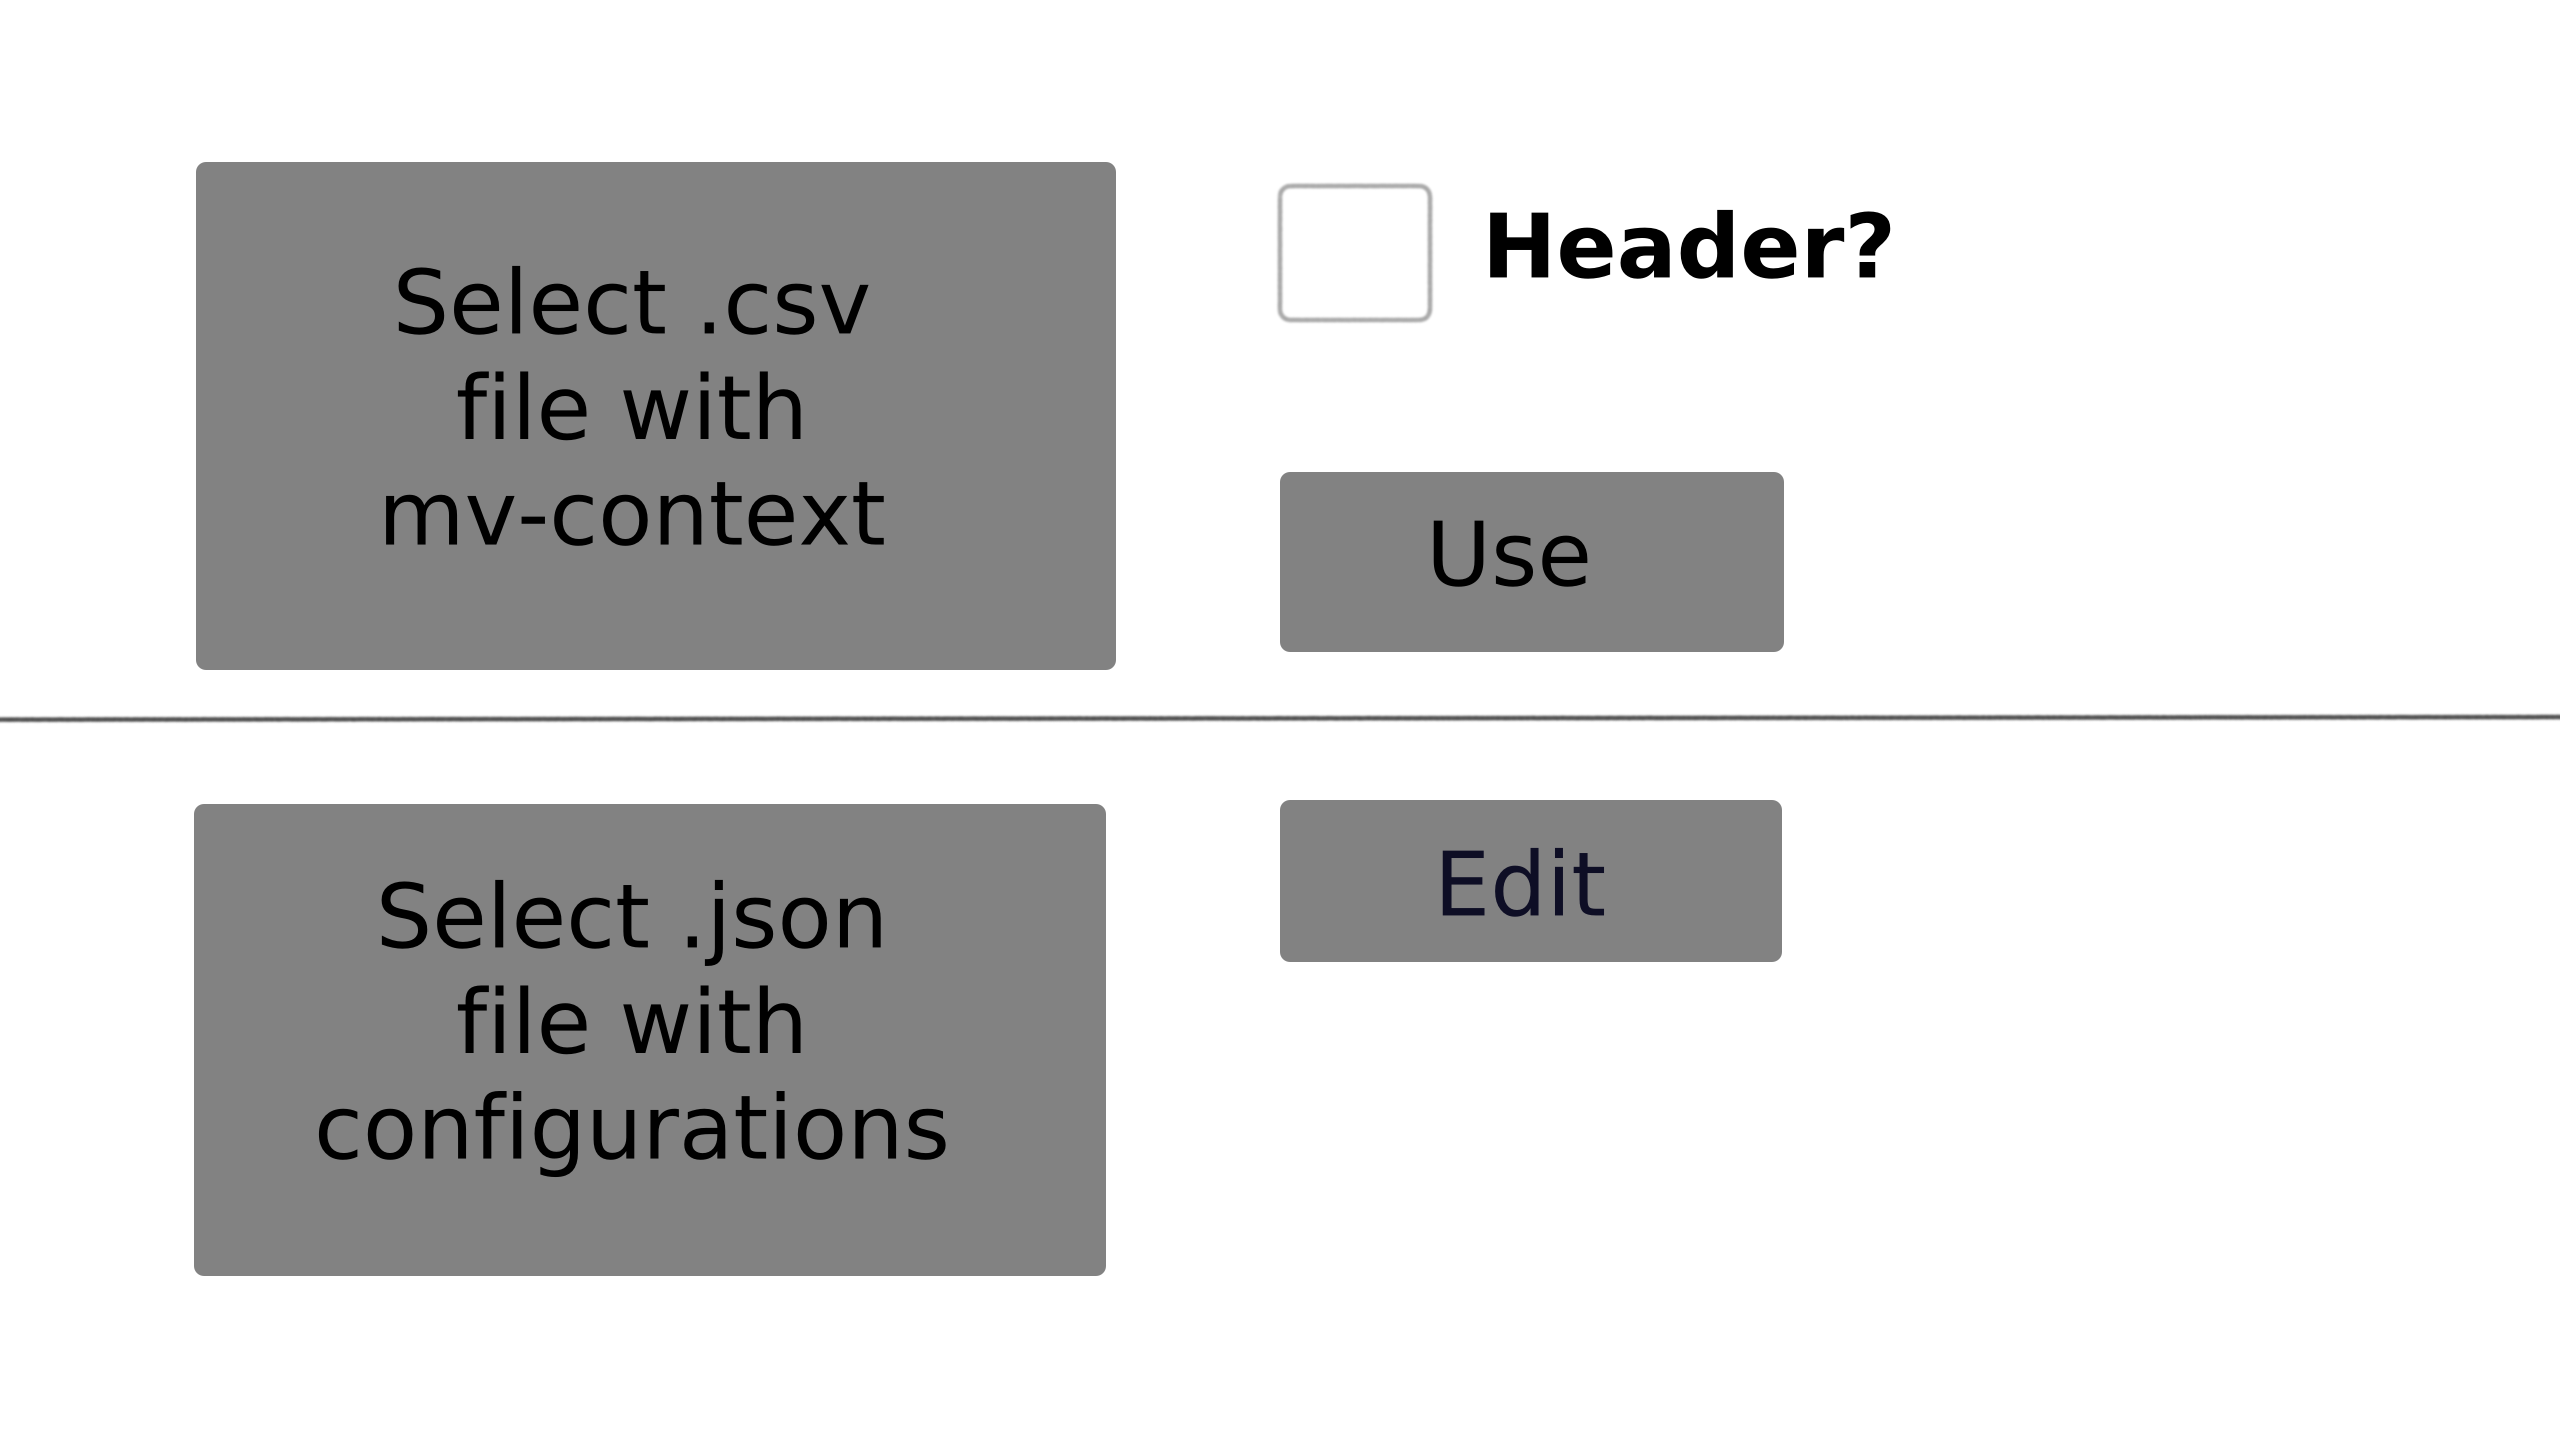
\includegraphics[width=\linewidth]{panel-1.png}
	\caption{The panel to select files (both versions)}
	\label{fig:p1}
\end{figure}

\subsection{Features}
\begin{itemize}
	\item Select any local .csv file with a mv-context
	\item Checkbox to mark existence of a header line
	\item Different input box to instead reuse a .json file with an old configuration
	\item Button to second panel
\end{itemize}

\newpage
\section{Panel}
\begin{figure}[H]
	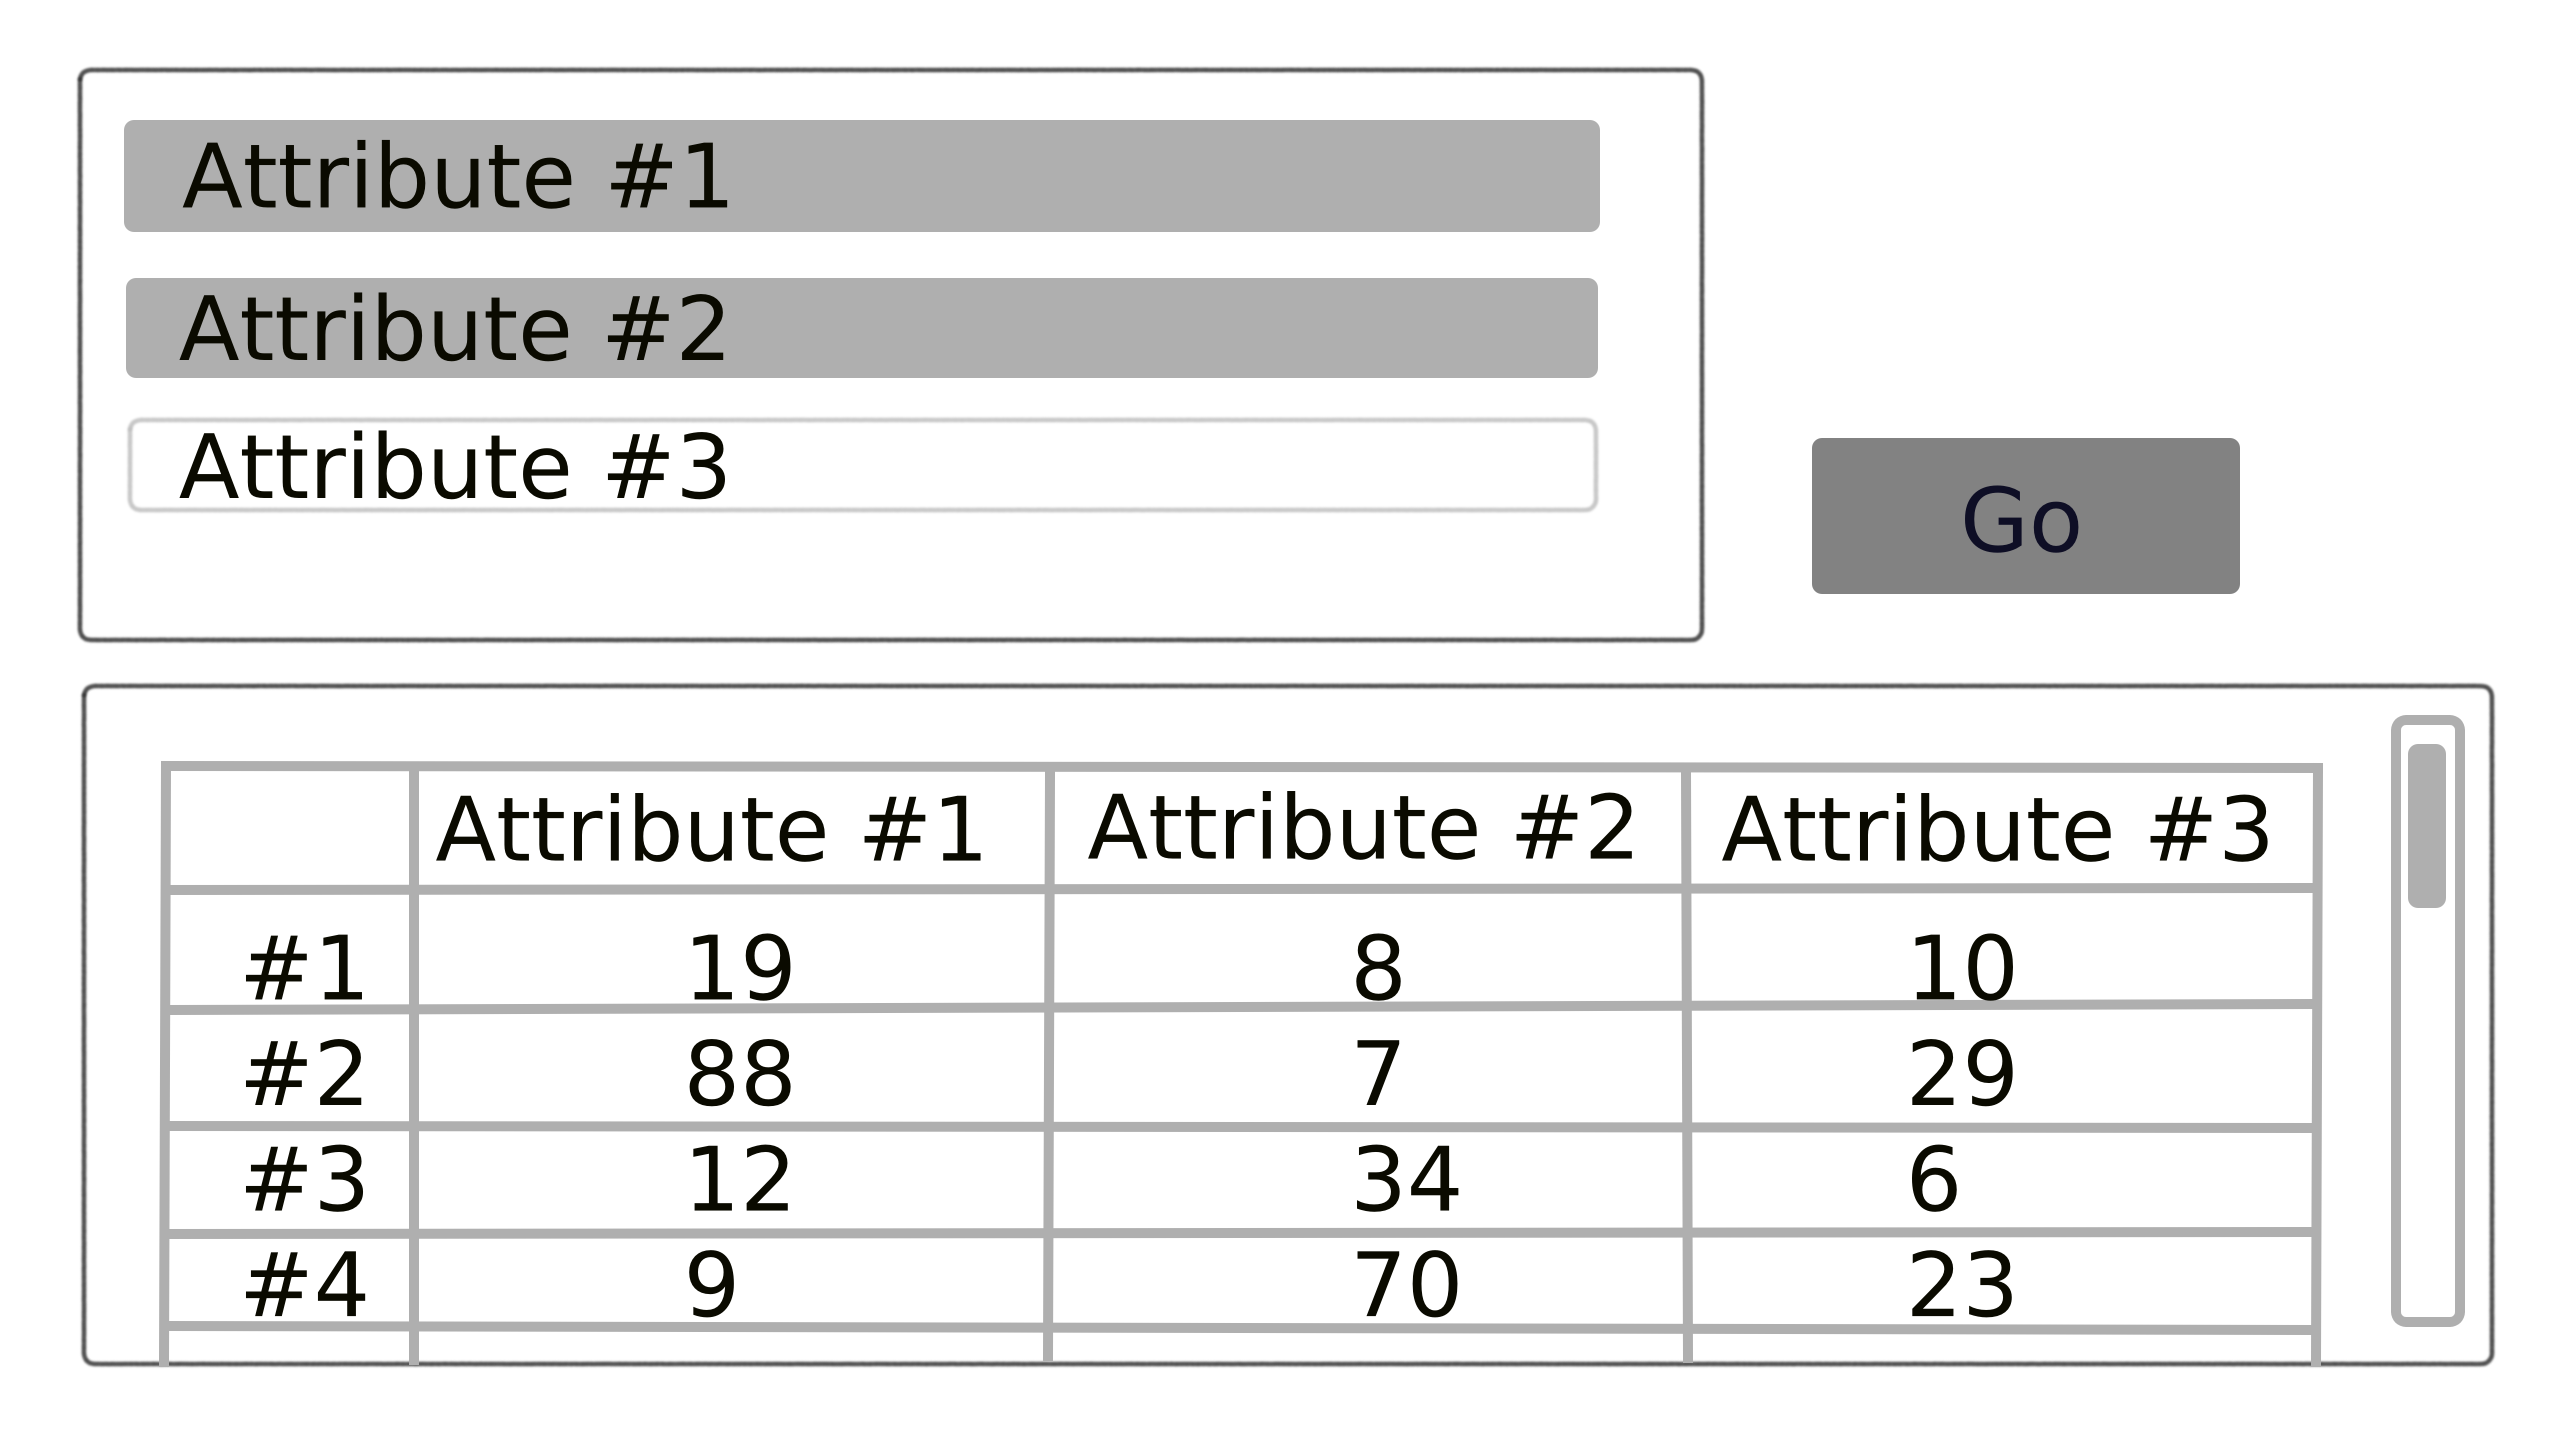
\includegraphics[width=\linewidth]{panel-2.png}
	\caption{Preselection panel}
	\label{fig:p2}
\end{figure}

\subsection{Features}
\begin{itemize}
	\item Select all Attributes (multi-select input) to scale (gray) and to exclude (white)
	\item Preview of the context in scroll-able box (x and y axis)
	\item Button to third panel
\end{itemize}

\newpage
\section{Panel}
\begin{figure}[H]
	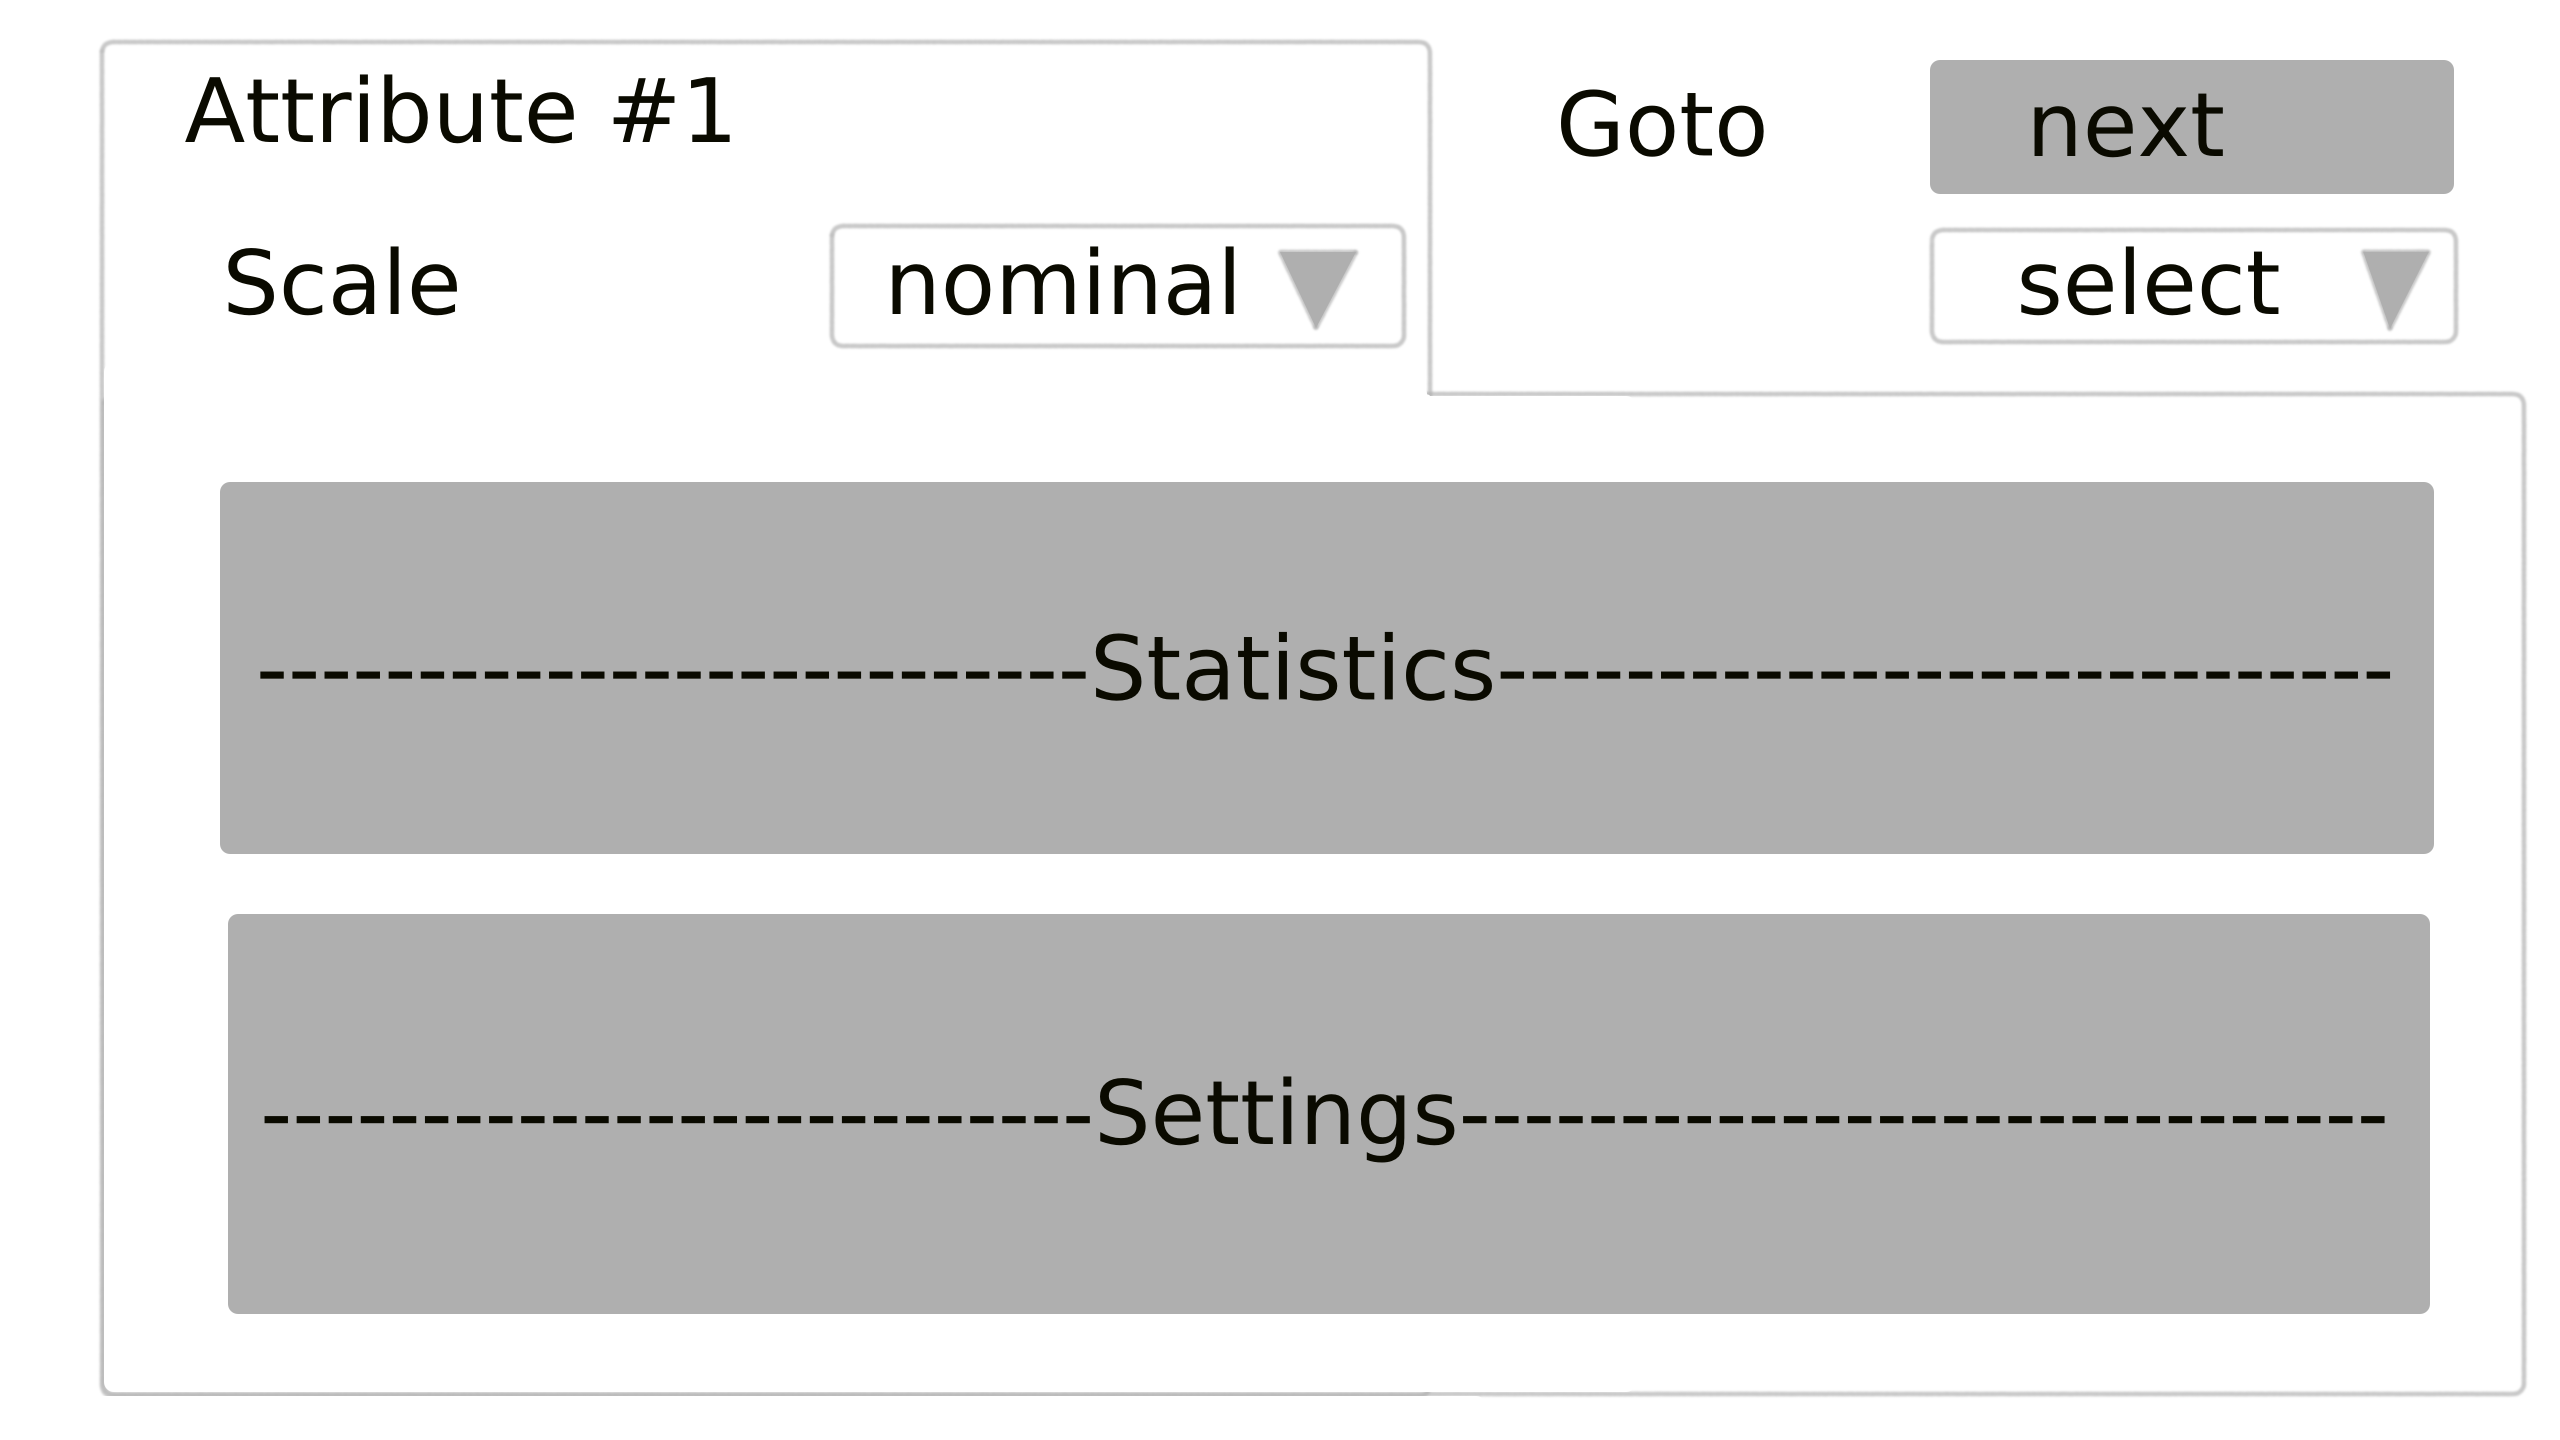
\includegraphics[width=\linewidth]{panel-3.png}
	\caption{Scaling panel}
	\label{fig:p2}
\end{figure}
\begin{itemize}
	\item Preselected scaling option for each attribute
	\item Option to choose different measurement levels (ordinal and numeric)
	\item Descriptive statistics for values of each attribute
	\item Settings to change scaling
	\item Button to iterate attributes
	\item Selection to jump between attributes
\end{itemize}

\subsection{Statistics}
\begin{figure}[H]
	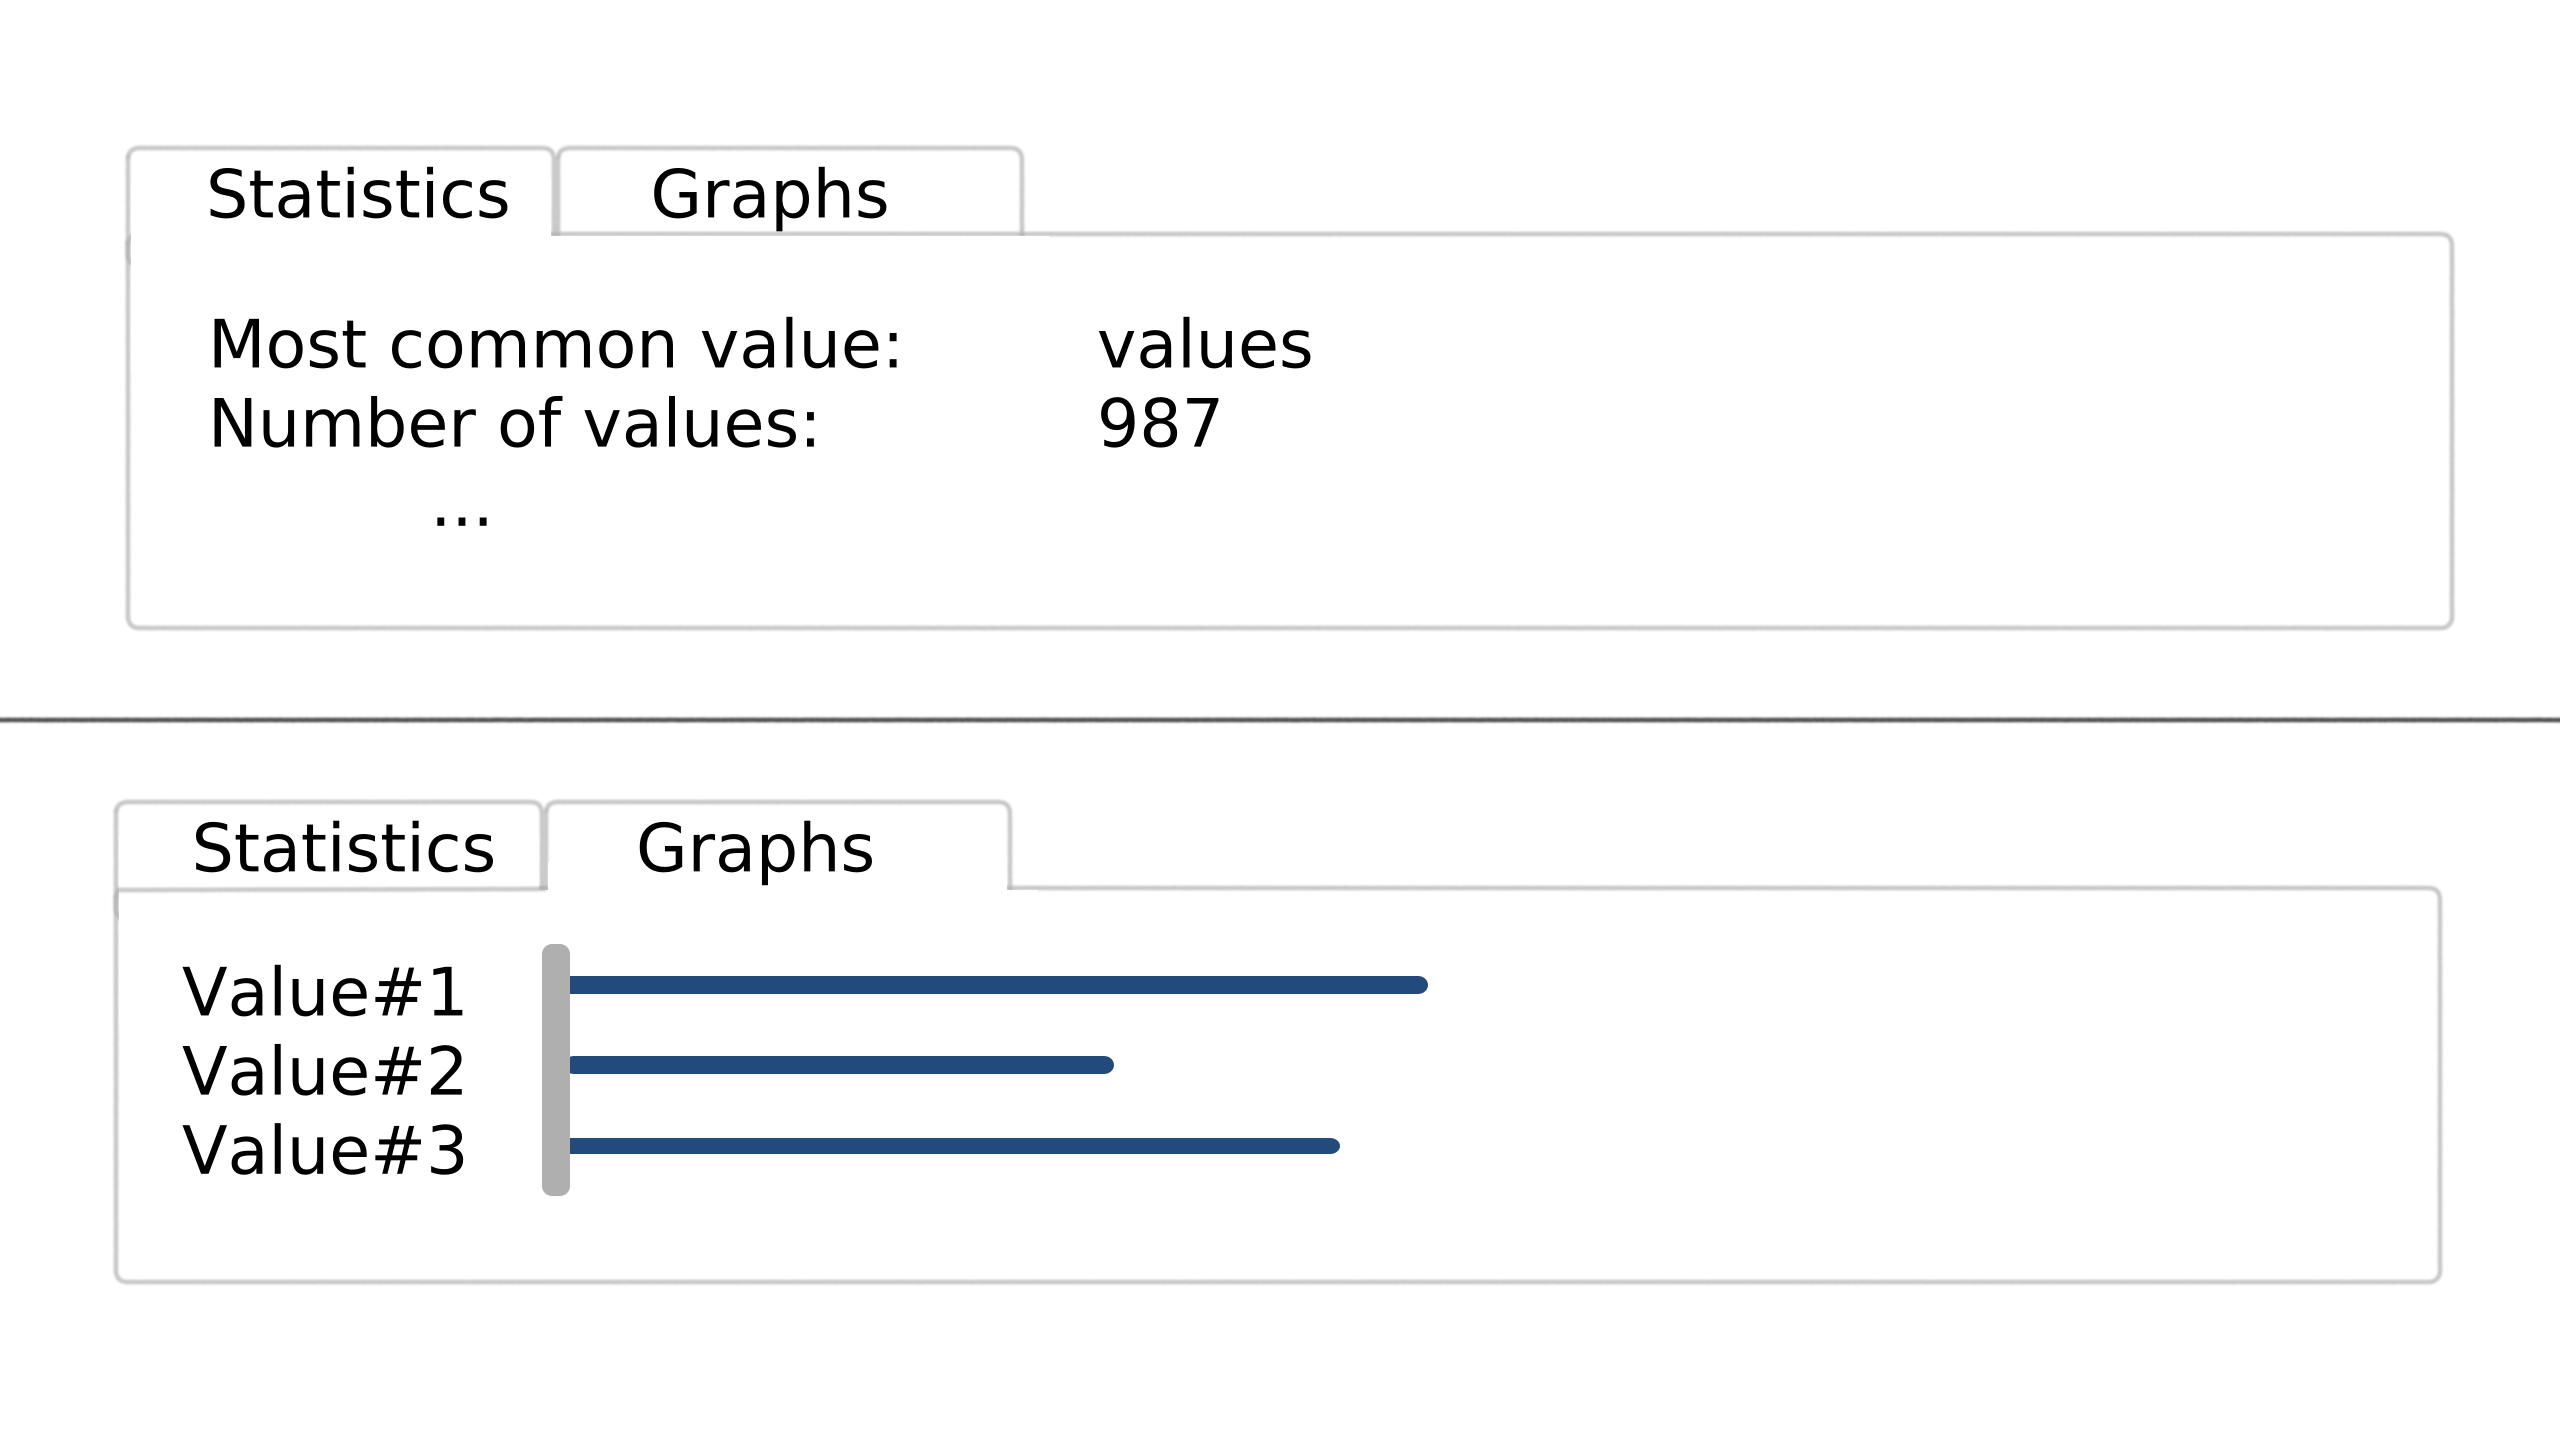
\includegraphics[width=\linewidth]{stat.png}
	\caption{Statistics panel}
	\label{fig:s1}
\end{figure}
\begin{itemize}
	\item Based on data type and measure: mean, median, list of all values , most common element etc.
	\item Distribution graphs
\end{itemize}

\newpage
\subsection{Settings}
\begin{itemize}
	\item Nominal
		\begin{itemize}
		\item Entirely automatic
		\end{itemize}	    
	\item Ordinal
		\begin{figure}[H]
			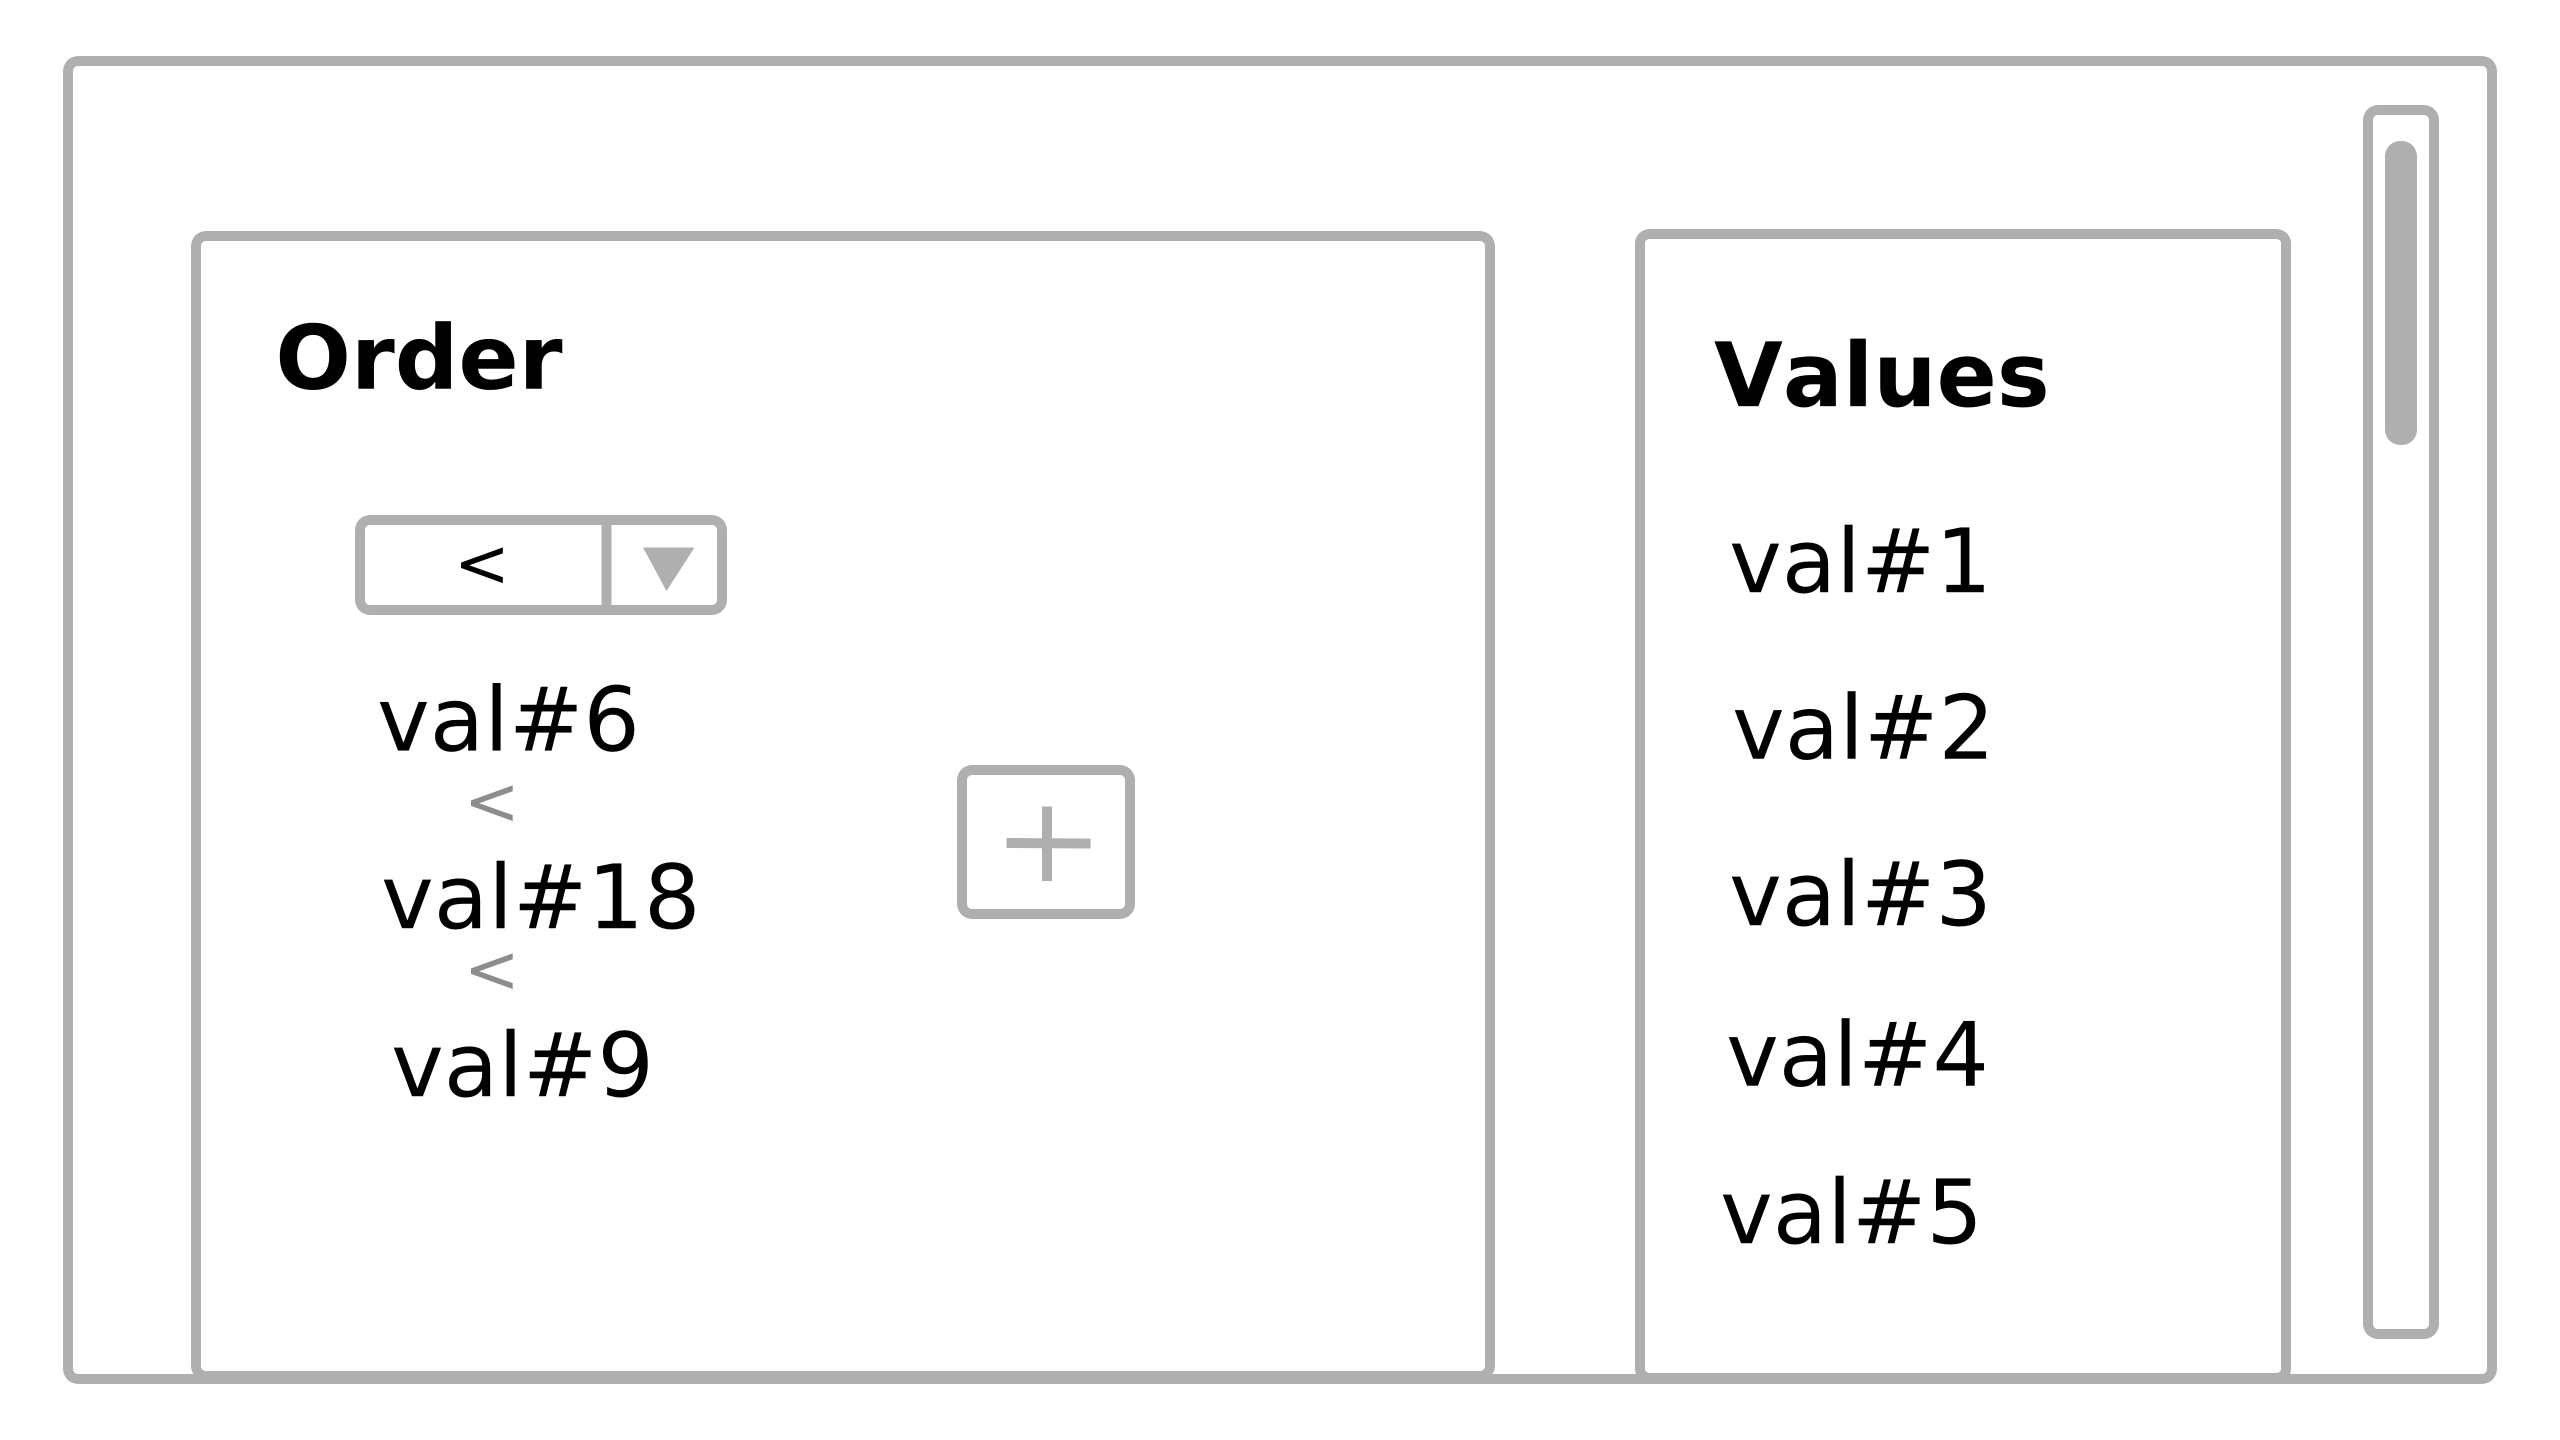
\includegraphics[width=\linewidth]{ord-2.png}
			\caption{Drag and Drop Version}
			\label{fig:o1}
		\end{figure}
		\begin{itemize}
			\item Sort values with drag and drop
			\item Different incomparable groups
			\item Different types of order
			\item All unused values are scaled nominally 
		\end{itemize}
		\begin{figure}[H]
			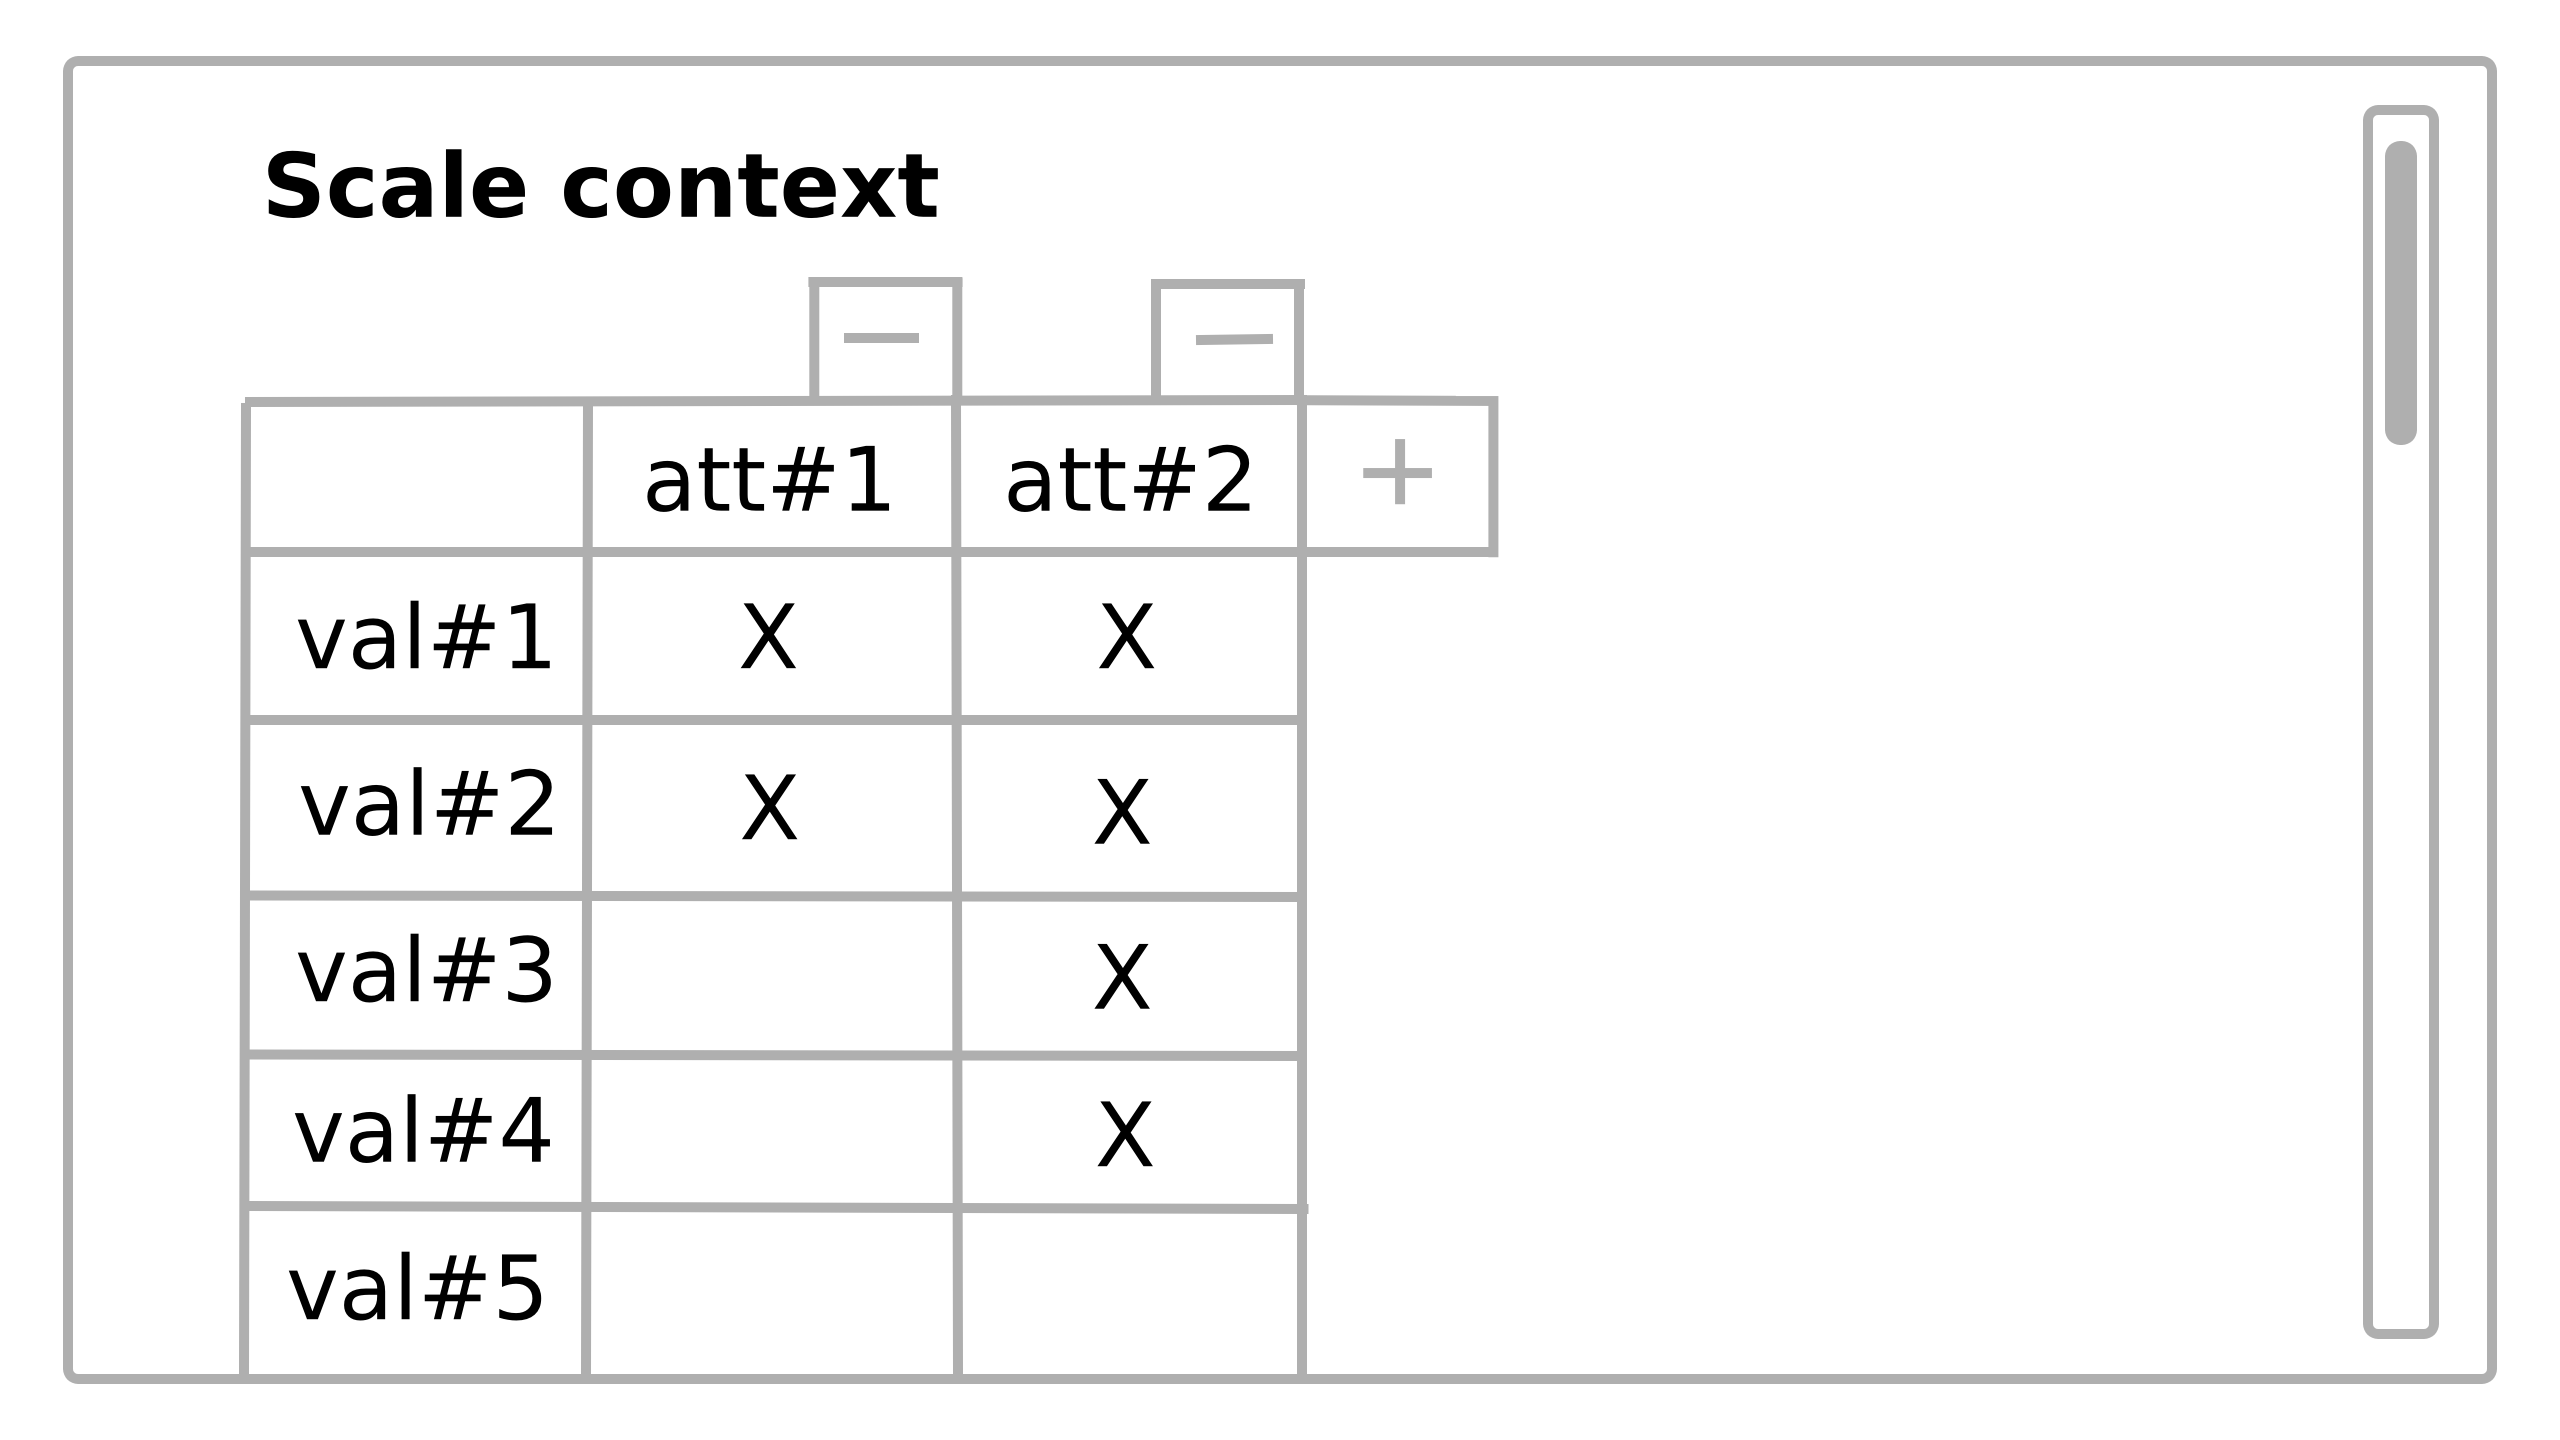
\includegraphics[width=\linewidth]{ord-1.png}
			\caption{Custom context}
			\label{fig:o2}
		\end{figure}
		\begin{itemize}
			\item Option to edit scale context directly
			\item Add and remove rows
		\end{itemize}
	\item Numeric
		\begin{figure}[H]
			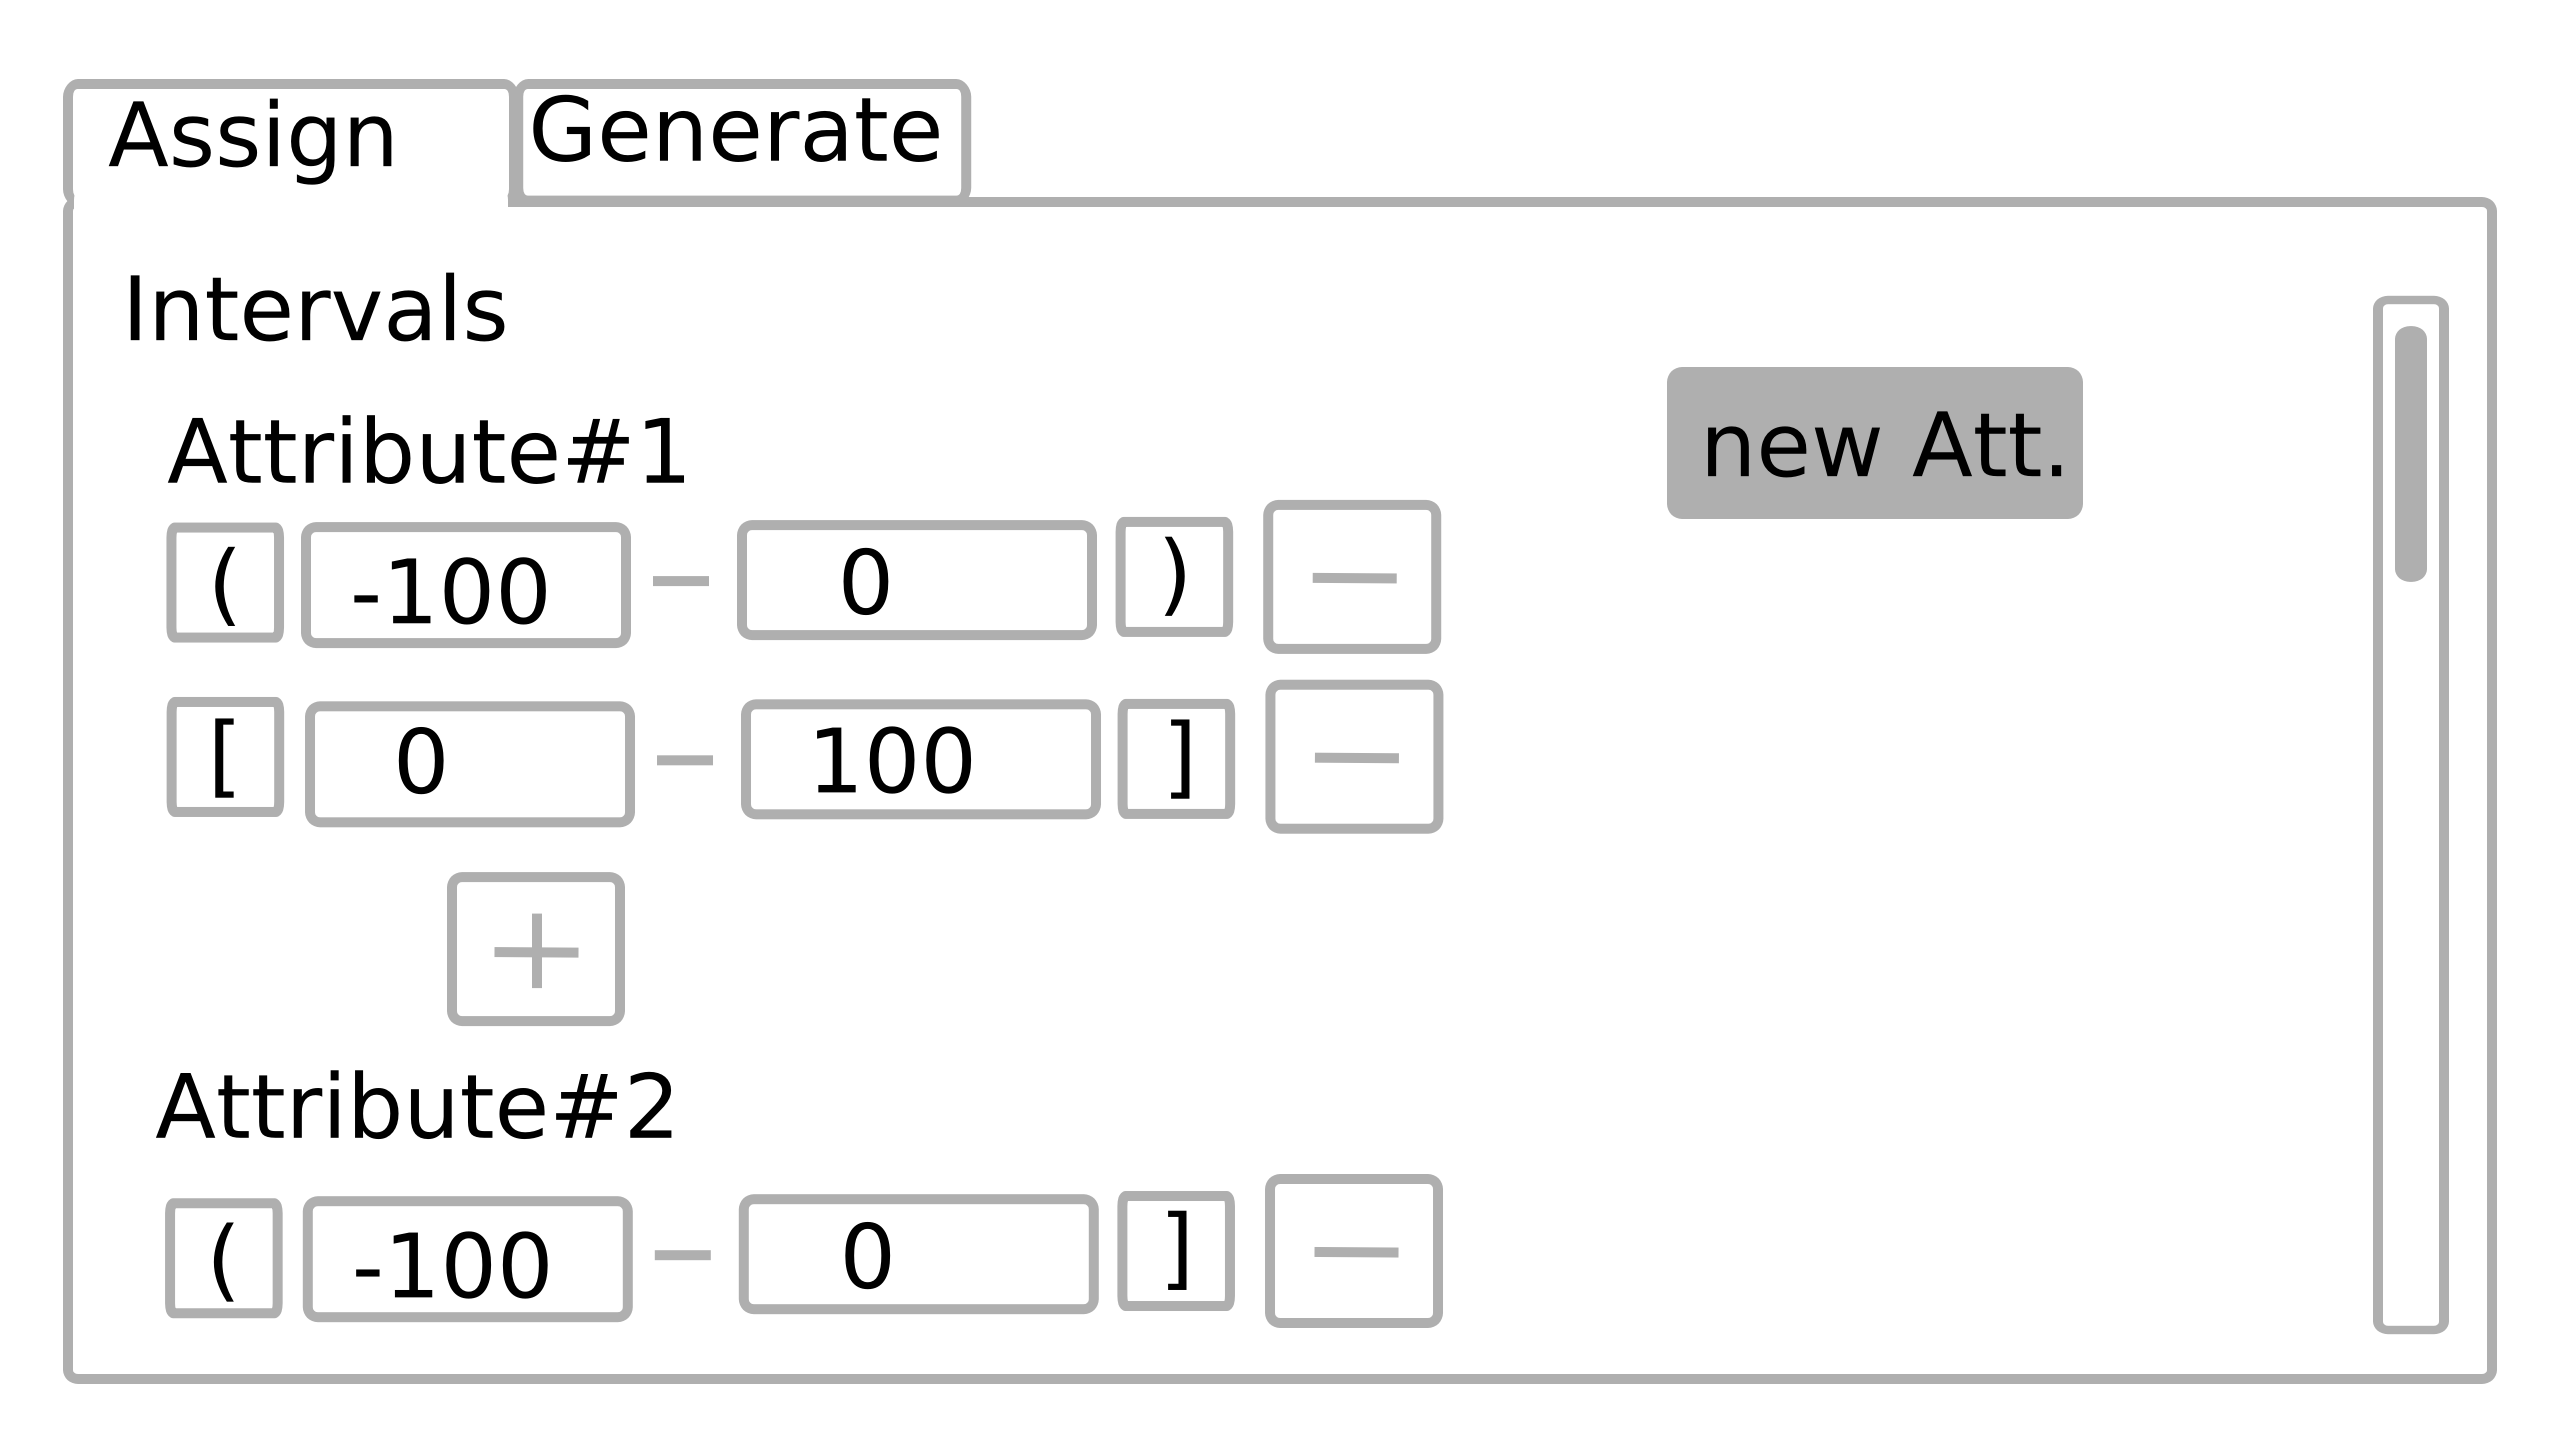
\includegraphics[width=\linewidth]{num.png}
			\caption{Custom intervals}
			\label{fig:n1}
		\end{figure}
	    \begin{itemize}
	    	\item Use predefined intervals with custom amount
	    	\begin{figure}[H]
	    		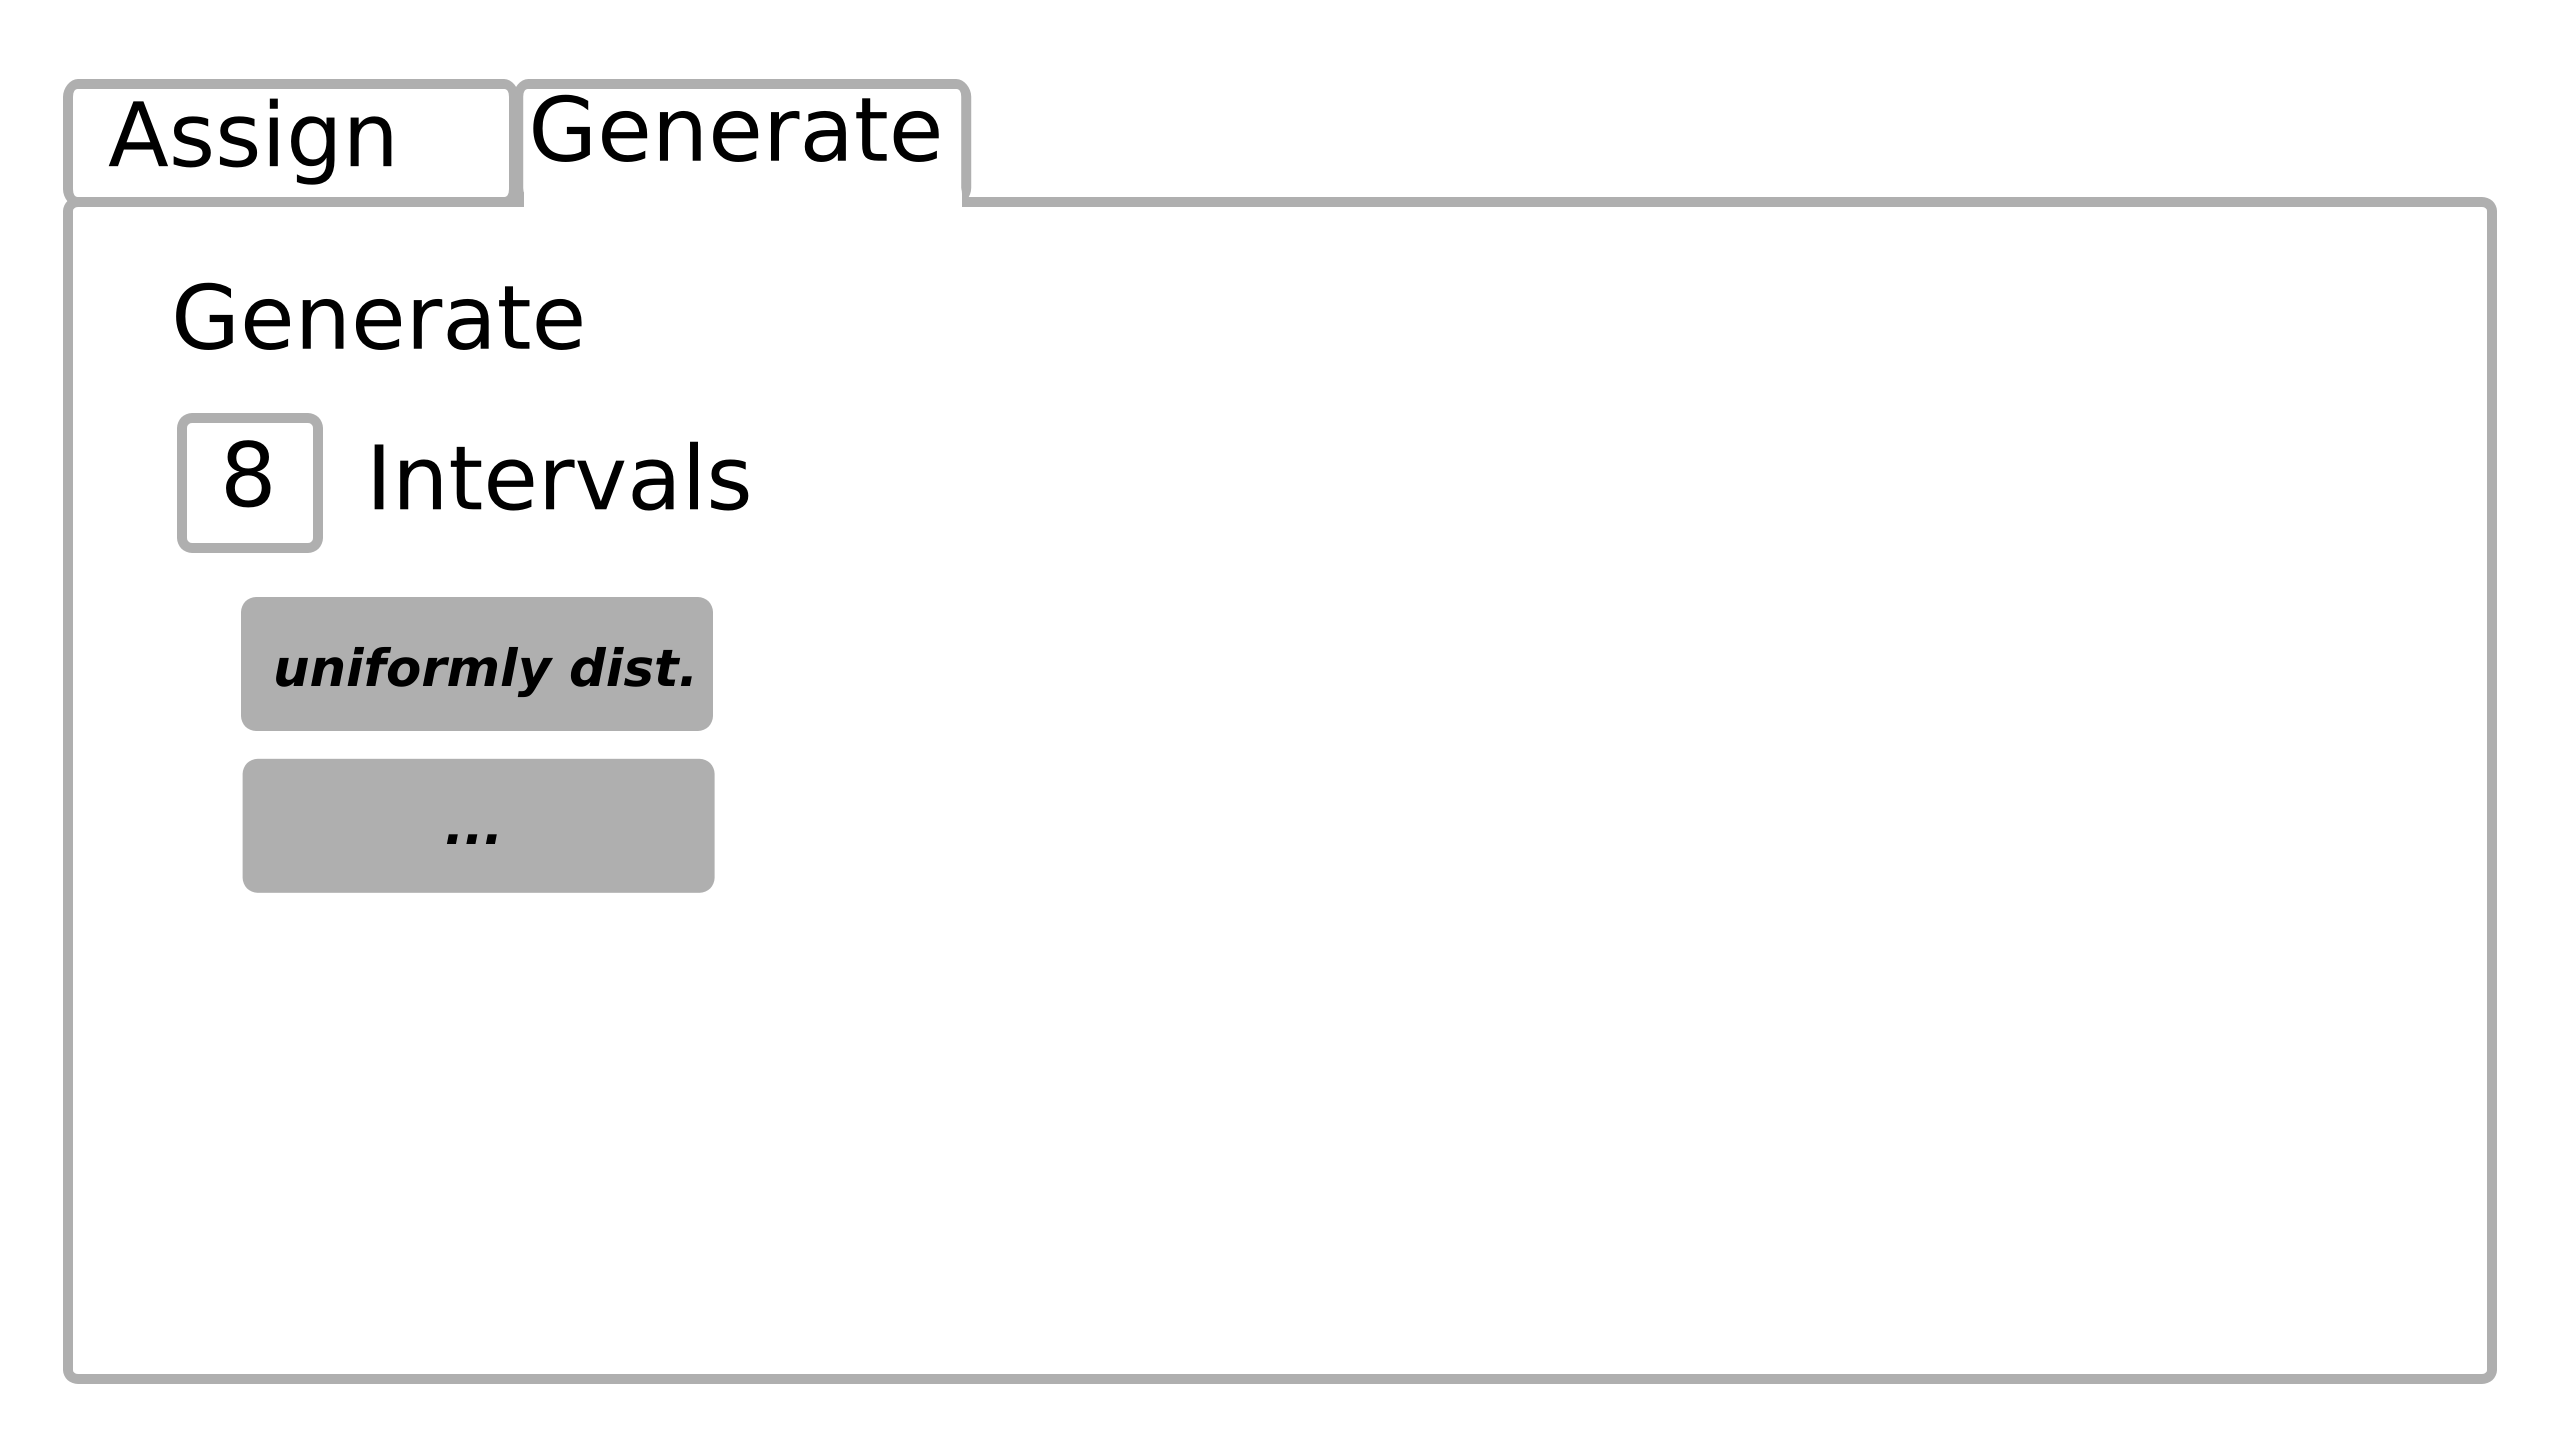
\includegraphics[width=\linewidth]{num_gen.png}
	    		\caption{Generate predefined intervals}
	    		\label{fig:n1}
	    	\end{figure}
	    	\item Generate custom intervals
	    \end{itemize}
\end{itemize}

\subsection{Export}
	\begin{itemize}
		\begin{figure}[H]
			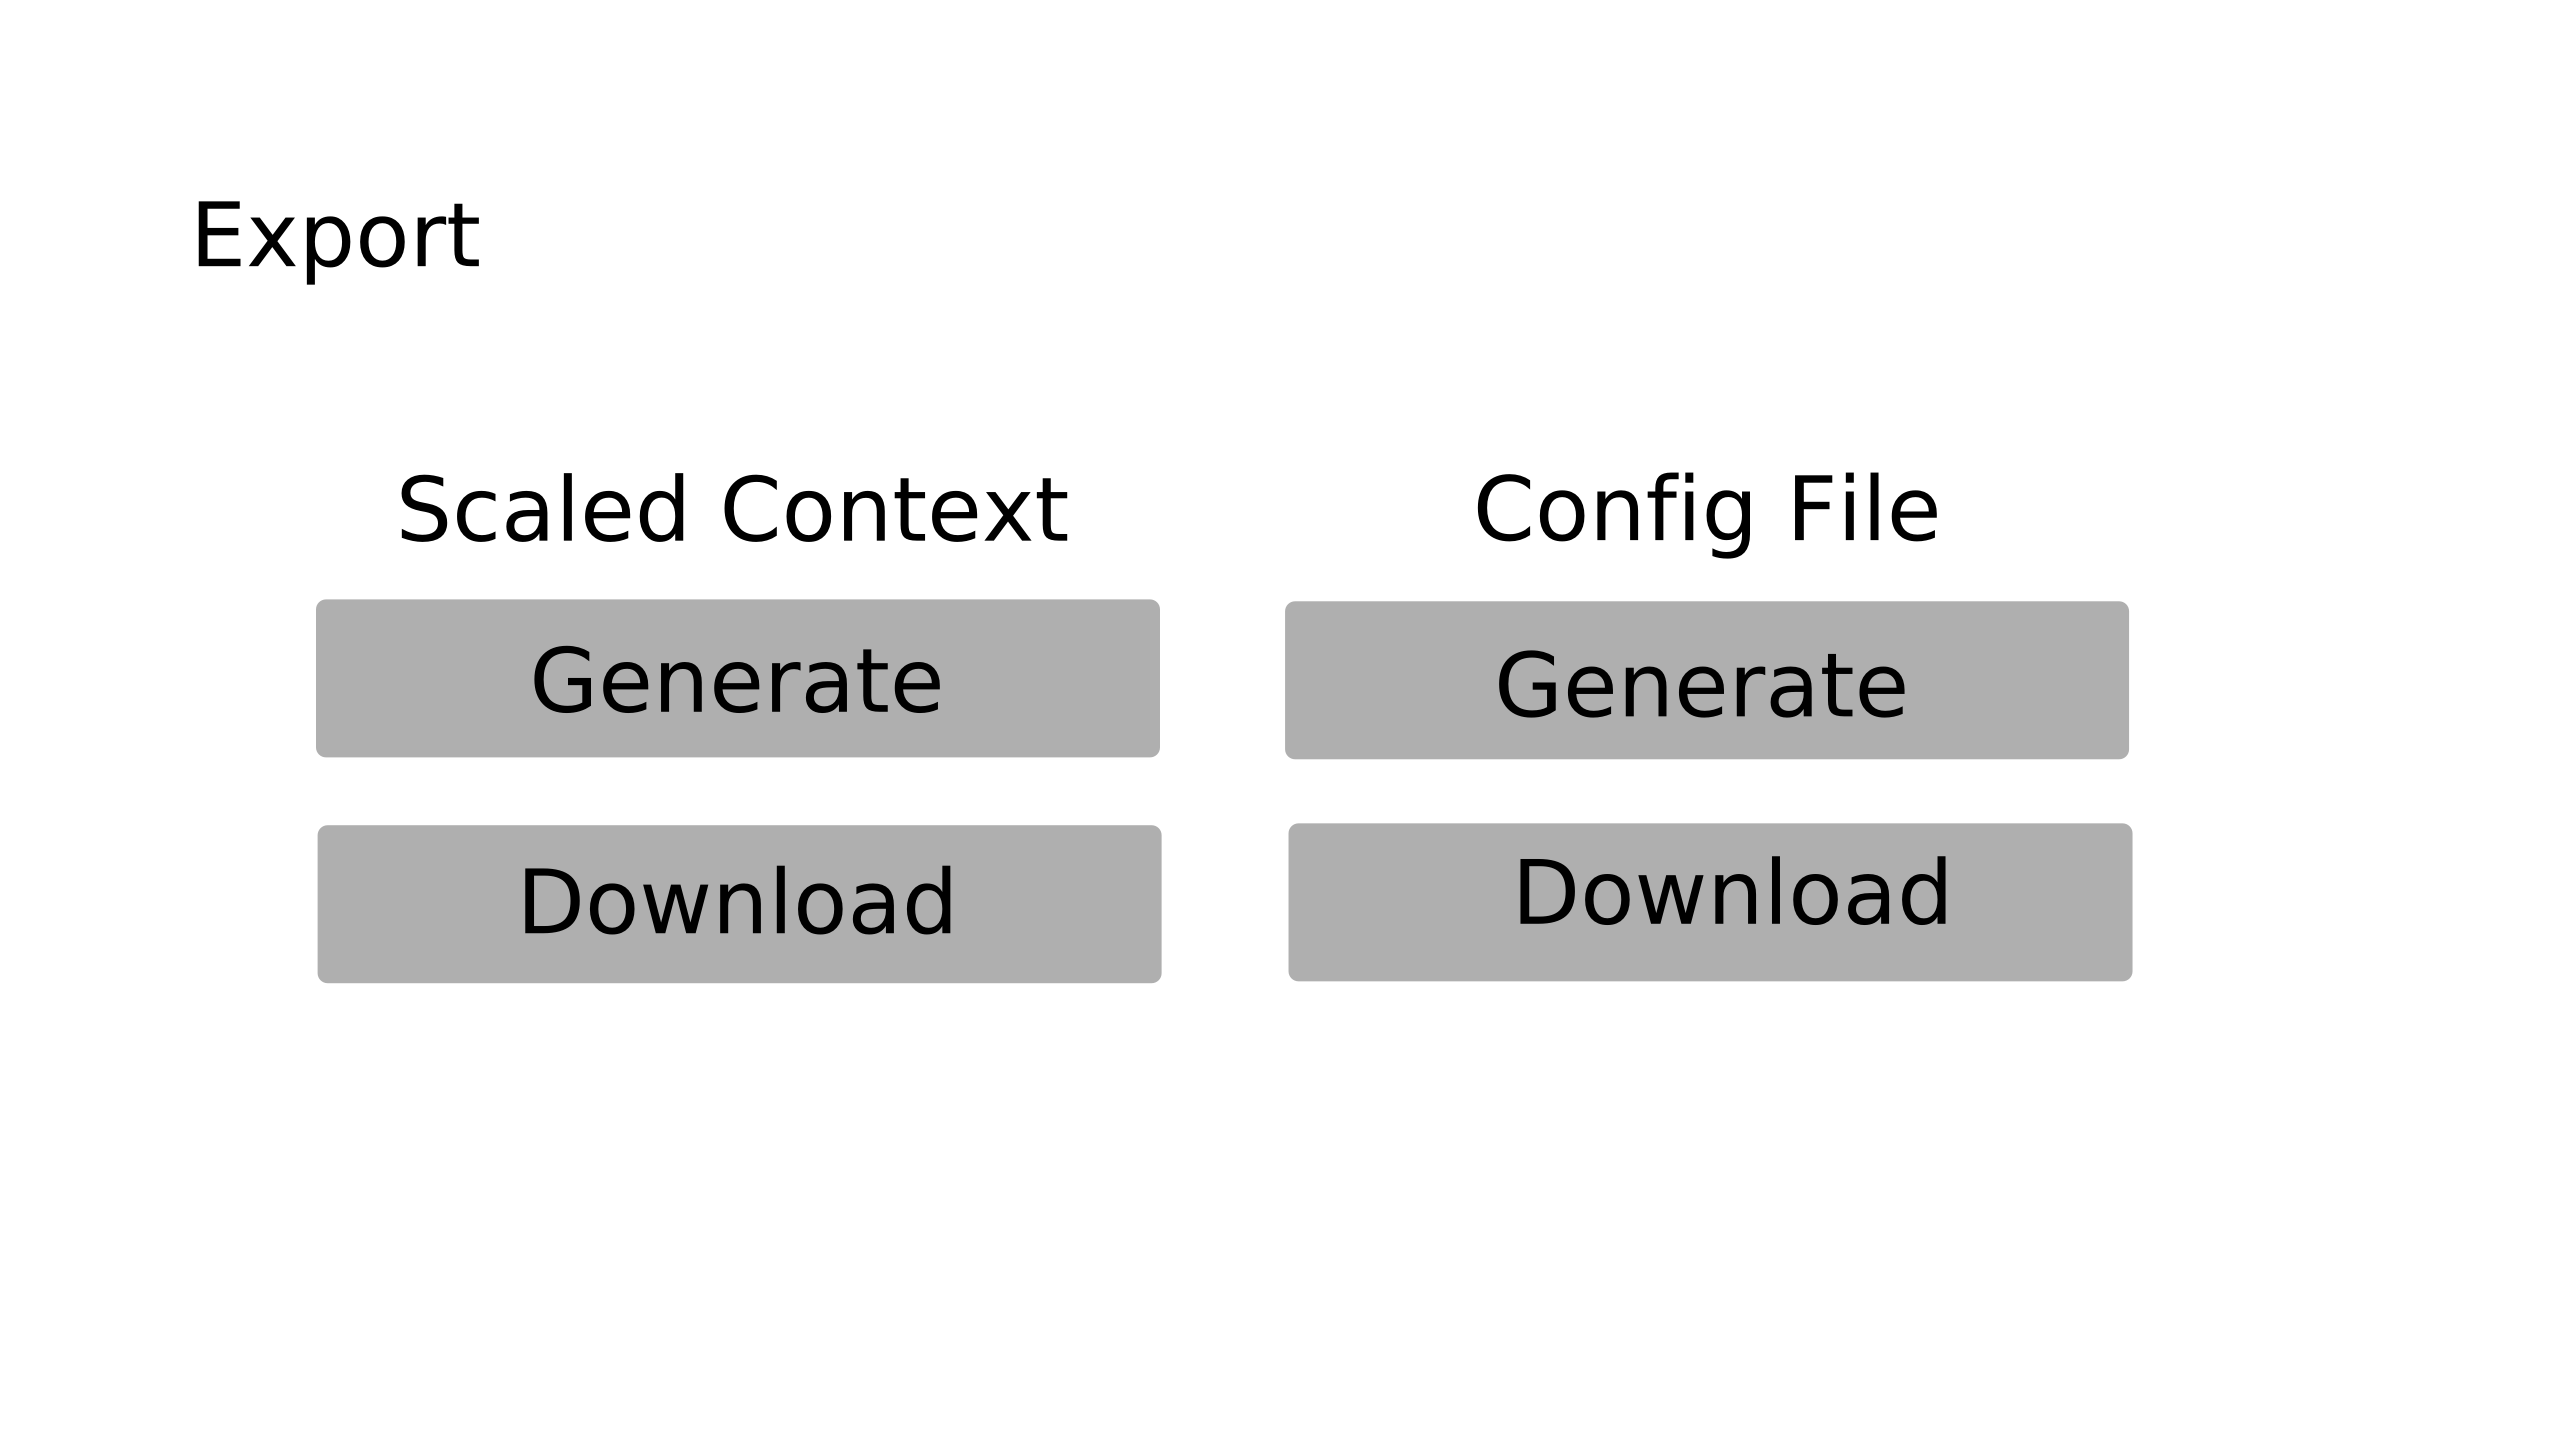
\includegraphics[width=\linewidth]{export.png}
			\caption{Export panel}
			\label{fig:n1}
		\end{figure}
		\item Apply scales to mv-context and download it
		\item Context in Burmeister format
		\item Option to download .json config file to edit the scaling later
	\end{itemize}

\end{document}
